\ifdefined\isprintversion
\else
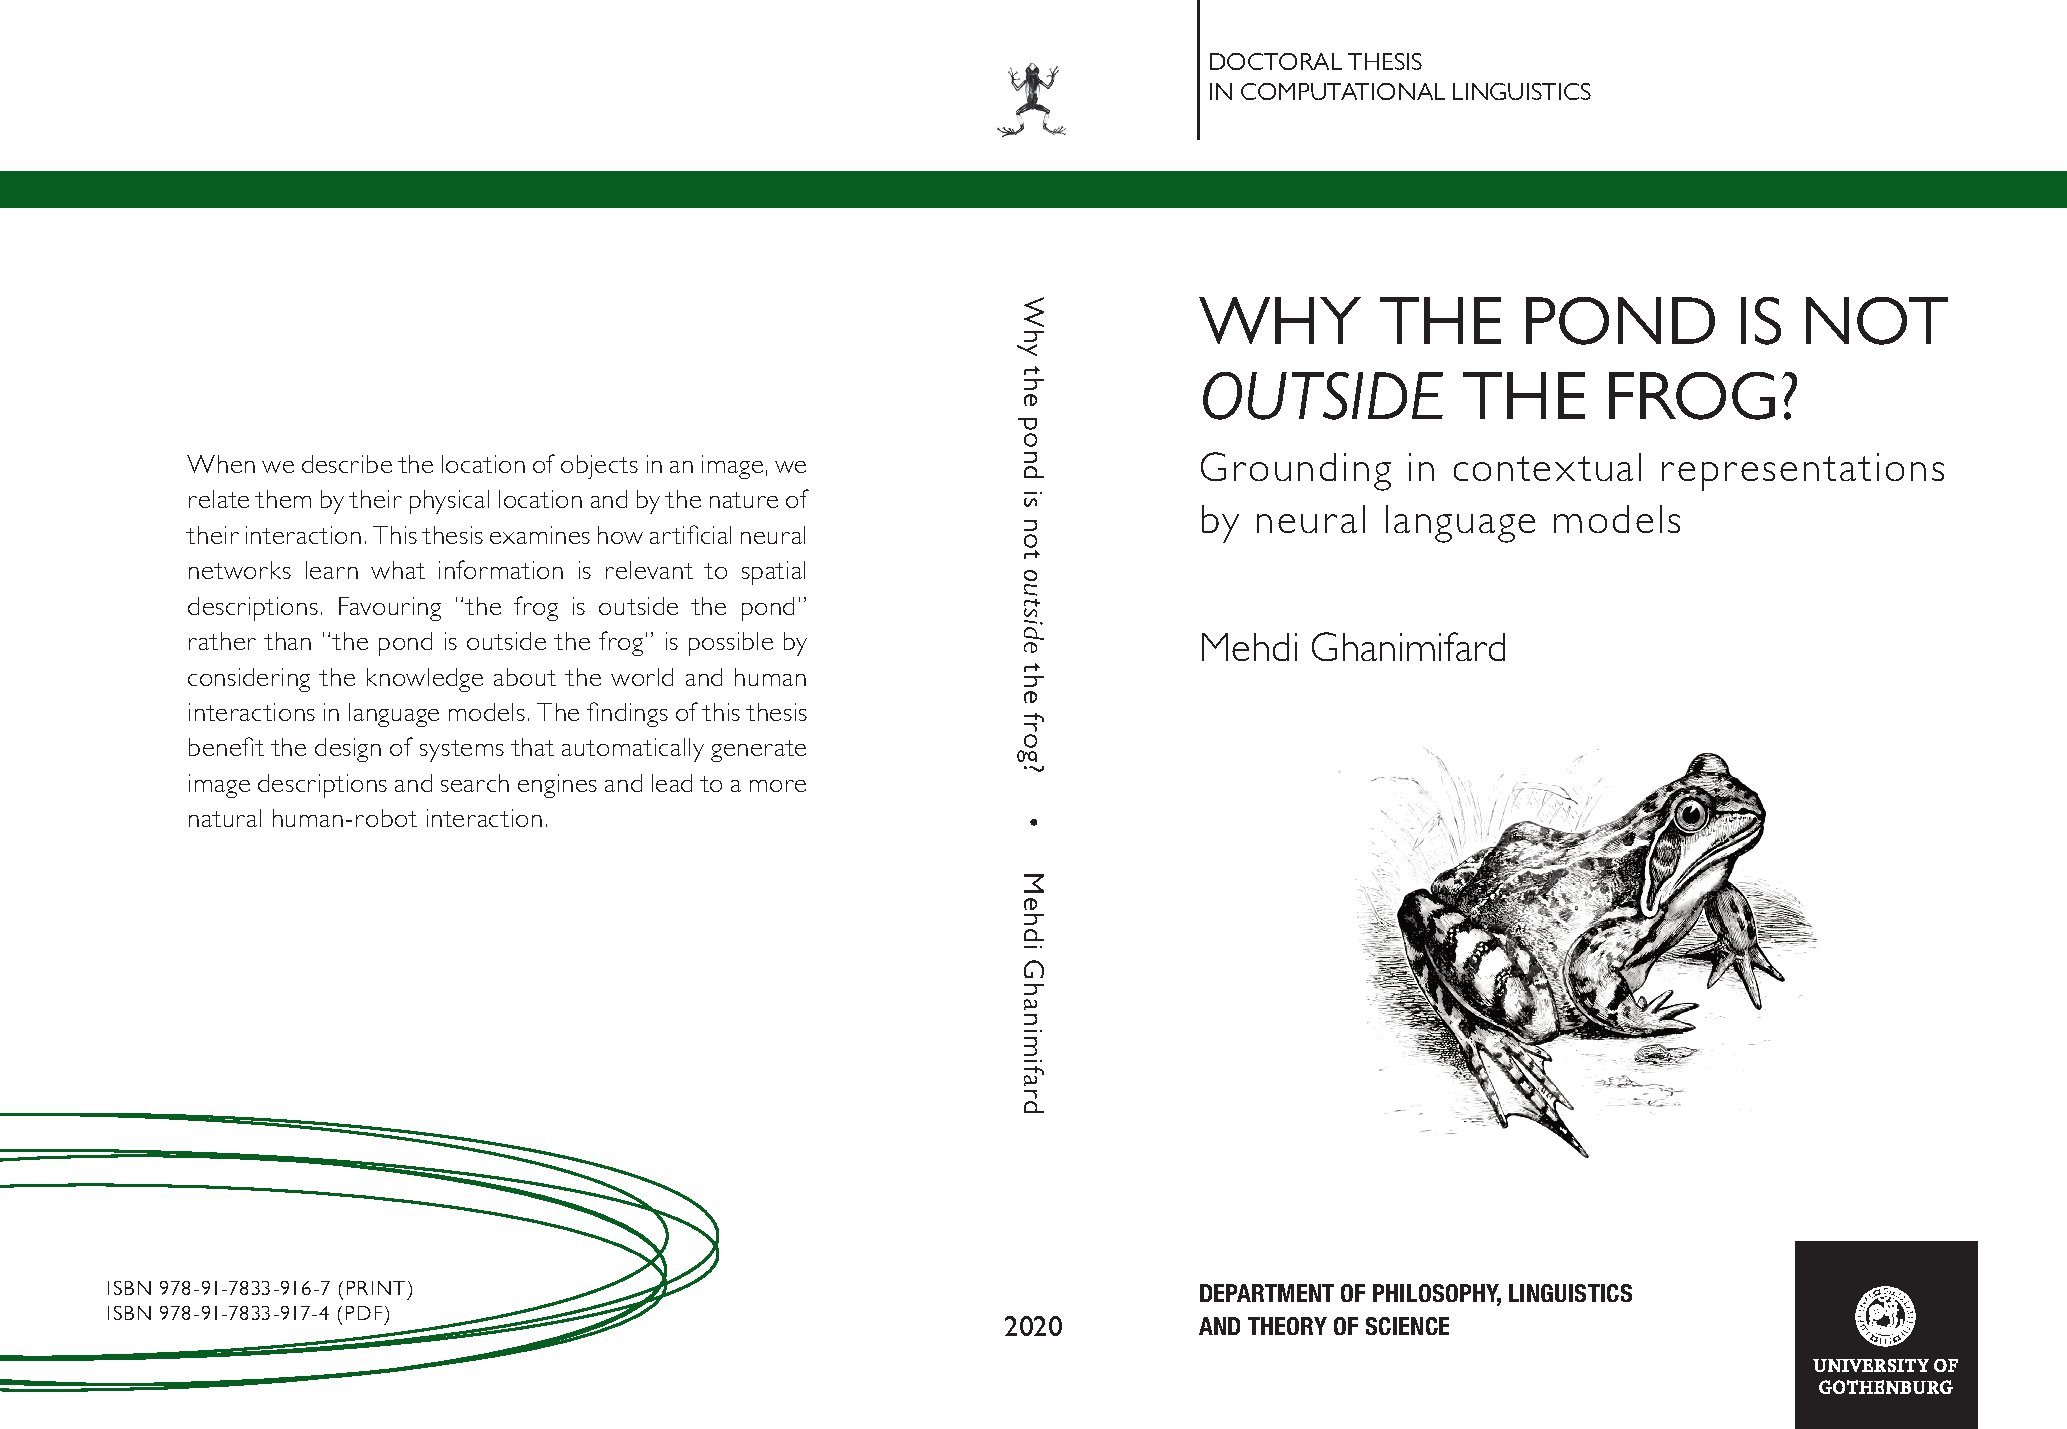
\includepdf[fitpaper,trim=185mm 0mm 0mm 0mm]{gfx/cover/cover-digital.pdf}
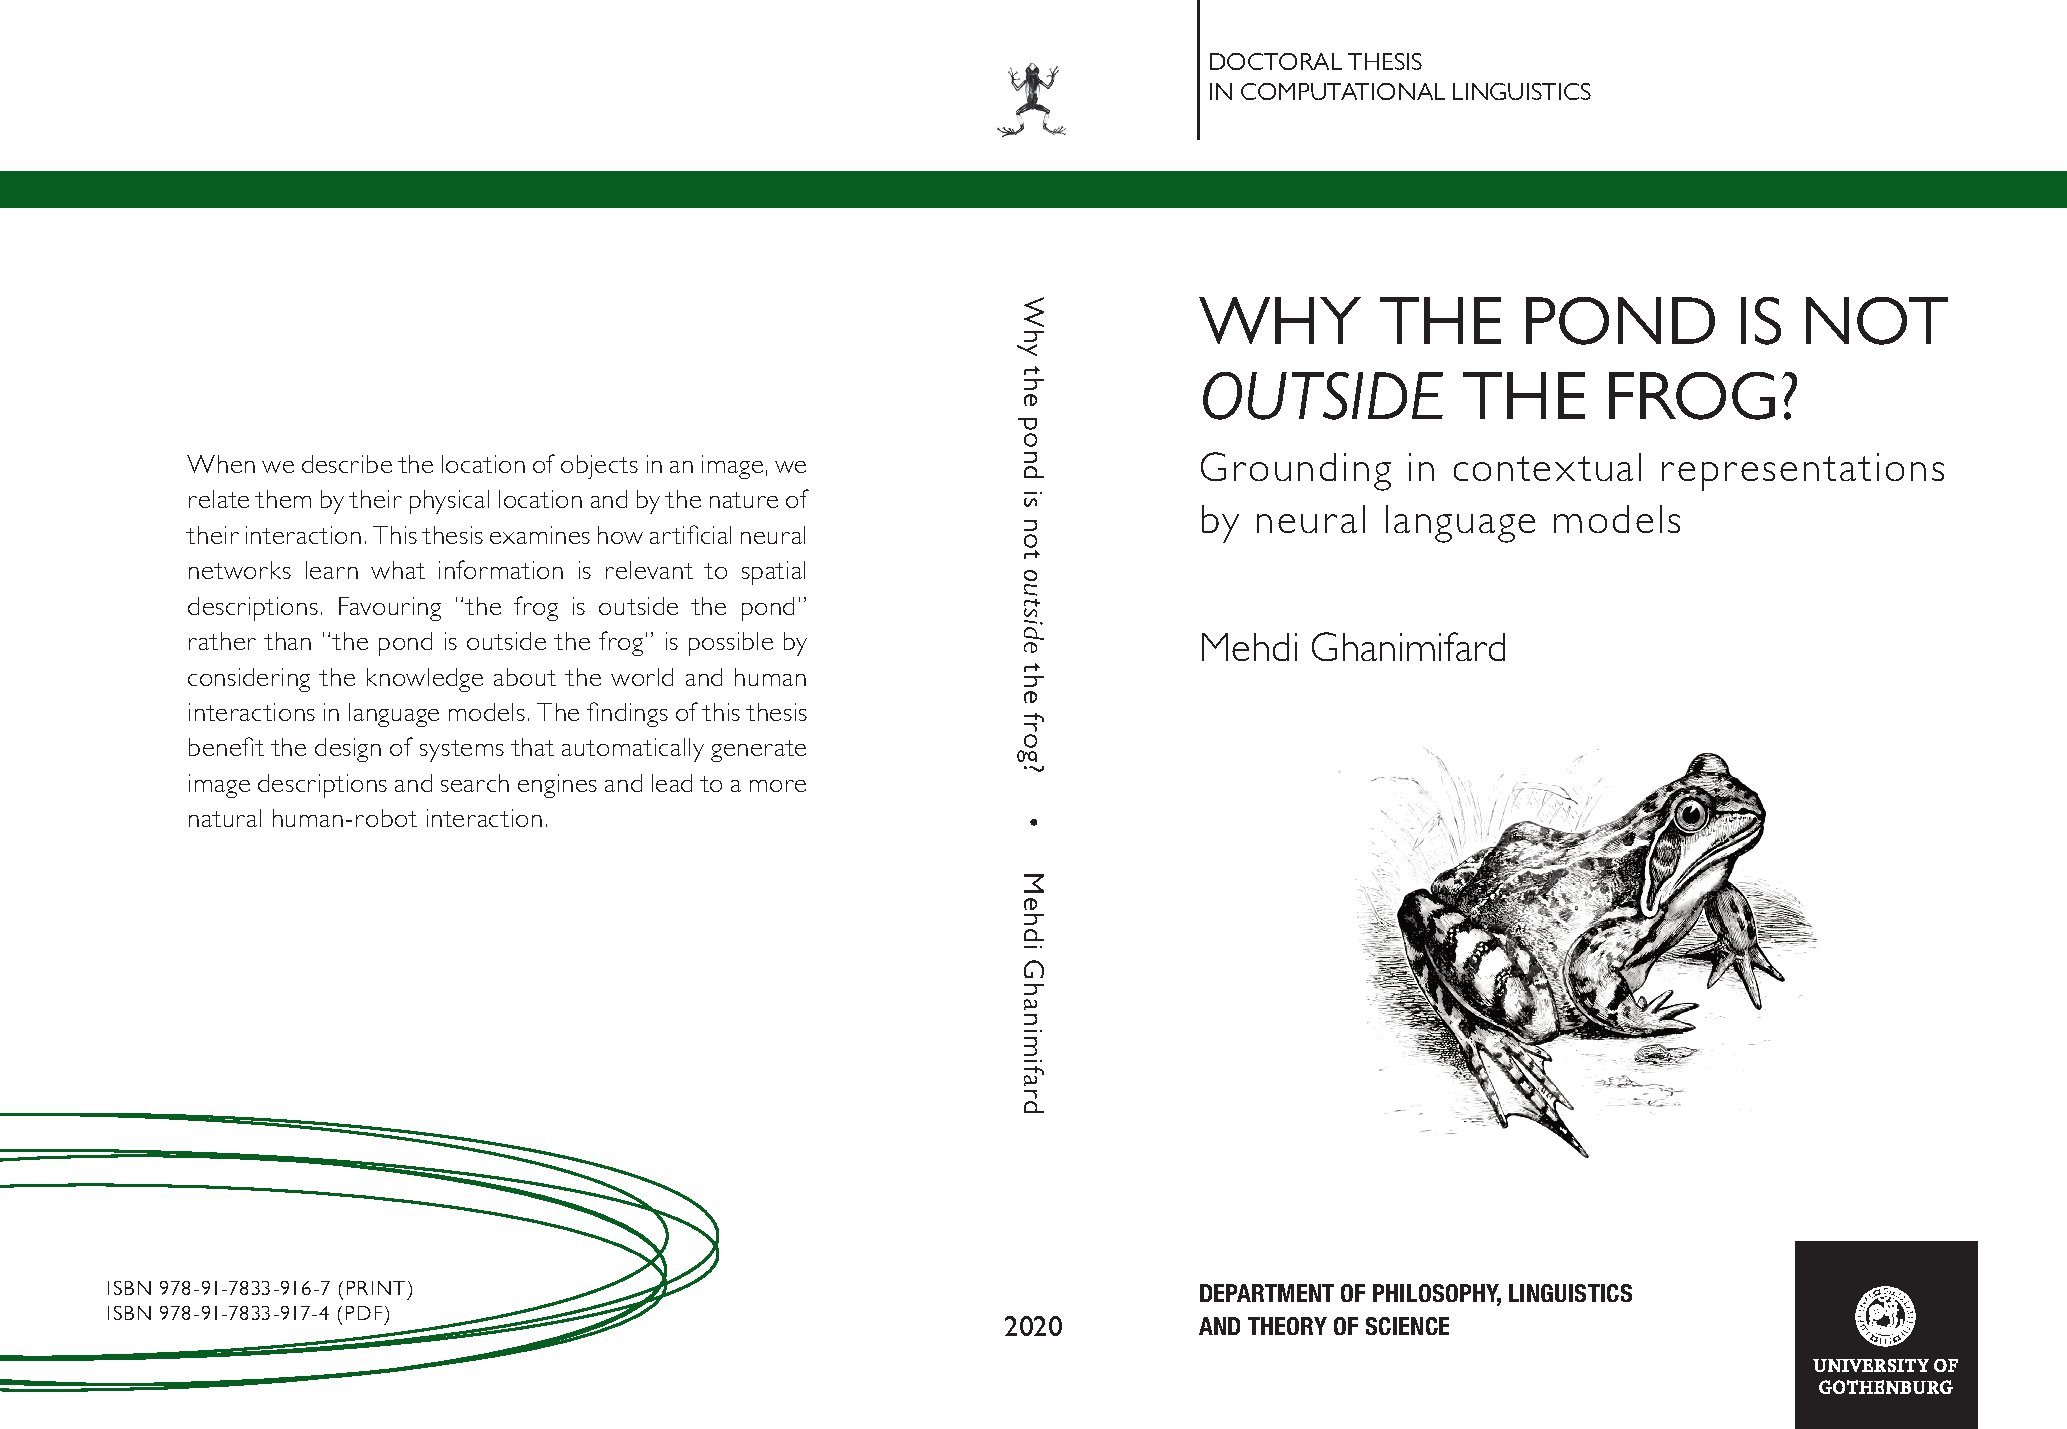
\includepdf[fitpaper,trim=0mm 0mm 185mm 0mm]{gfx/cover/cover-digital.pdf}
\setcounter{page}{1}
\fi

\begin{titlepage}
	\pdfbookmark[0]{Cover}{Cover}
	\flushright
	\hfill
	\vfill
	{\centering\LARGE\tgherosfont\thesisTitle \par}
	\vfill
	\flushright
\end{titlepage}


\begin{titlepage}
	\pdfbookmark[0]{Titlepage}{Titlepage}
	\tgherosfont
	\centering

	\vfill
	{\large\thesisSubject} \\[5mm]
	{\LARGE\thesisTitle \\[25mm]}
	
	\vfill
	
	{\Large \thesisName} \\[55mm]

	\vfill
	\textsf{\thesisUniversityDepartment} \\
	\textsf{\thesisUniversityGroup} \\ [10mm]
	\vfill

\includegraphics[width=6cm]{gfx/gu/LO_GUeng_cenSV.eps} \\
\thesisDate \\

\end{titlepage}


\hfill
\vfill
{
	\small
	\textbf{\thesisName} \\
	\textit{\thesisTitle} \\
	\thesisSubject, \thesisDate \\
	Main supervisor: \thesisFirstSupervisor \\[1.5em]
	\textbf{\thesisUniversity} \\
	\thesisUniversityDepartment \\
	\thesisUniversityStreetAddress \\[1.5em]
	The cover drawing from `{The Common Frog}' by \cite{thecommonfrog1881}. Not in copyright, scanned at Harvard University, Museum of Comparative Zoology, Ernst Mayr Library. \\
	The cover designed by Boshra Khoshnevis \\[1.5em]
	The research reported in this thesis was supported by a grant from the Swedish Research Council (VR project 2014-39) for the establishment of the Centre for Linguistic Theory and Studies in Probability (CLASP) at the University of Gothenburg.\\[1.5em]
	ISBN: \thesisISBNPrint\ (PRINT) \\
	ISBN: \thesisISBNPDF\ (PDF) \\[1.5em]
	Part I of the publication is also available in full text at: \\
	\url{http://hdl.handle.net/2077/64095}
}
